\chapter{Fundamentação Teórica}
\label{cap:fundamentacao}

Este capítulo apresenta os conceitos de \english{\acrfull{csr}} e \english{\acrfull{ssr}}, abordando os princípios fundamentais do desenvolvimento web relacionados à renderização de conteúdo. Também são discutidos aspectos como \acrshort{seo}, desempenho, infraestrutura de serviços e impacto na experiência do usuário, estabelecendo a base teórica para o estudo de caso desenvolvido neste trabalho.

\section{\english{Client-Side Rendering} (\acrshort{csr})}
\label{subsec:csr}

A \textbf{\english{\acrfull{csr}}} é uma técnica em que a geração da interface e do conteúdo final ocorre diretamente no navegador do usuário, utilizando JavaScript\footnote{JavaScript é uma linguagem de programação interpretada utilizada para criar conteúdo dinâmico em páginas web.}. Nessa abordagem, o servidor envia um arquivo \english{\acrfull{html}} mínimo, contendo apenas a estrutura básica da página e referências a arquivos de estilo e scripts.{\cite{atori2024}}

Segundo \citeonline{atori2024}, o processo de renderização no cliente segue as seguintes etapas:

\begin{enumerate}
    \item O servidor envia uma página \acrshort{html} em branco contendo apenas links para os arquivos \english{\acrfull{css}} e JavaScript.
    \item O navegador interpreta o \acrshort{html} e constrói a árvore do \english{\acrfull{dom}}
    \item Os arquivos de estilo (\acrshort{css}) e script (JavaScript) são baixados pelo navegador.
    \item A aplicação é renderizada dinamicamente pelo JavaScript, incluindo elementos visuais como texto, imagens e botões.
    \item O conteúdo da página é atualizado de forma interativa conforme o usuário interage com a aplicação.
\end{enumerate}

Esse modelo é comumente utilizado em aplicações \english{\acrfull{spa}}, nas quais o carregamento inicial é seguido por atualizações dinâmicas sem recarregamento da página. Frameworks como React\footnote{React é uma biblioteca JavaScript para construção de interfaces de usuário, desenvolvida pelo Facebook.}, Vue.js\footnote{Vue.js é um framework JavaScript progressivo utilizado para a criação de interfaces web interativas, focado na camada de visualização.}, Angular\footnote{Angular é um framework para desenvolvimento de aplicações web, mantido pelo Google, que utiliza TypeScript como linguagem principal.} e Svelte\footnote{Svelte é um framework JavaScript que realiza a compilação de componentes no momento do build, gerando código otimizado sem a necessidade de um virtual DOM.} são amplamente utilizados para implementar \acrshort{csr}.

\begin{figure}[h!]
    \centering
    \caption{Etapas do método de renderização no lado do cliente}
    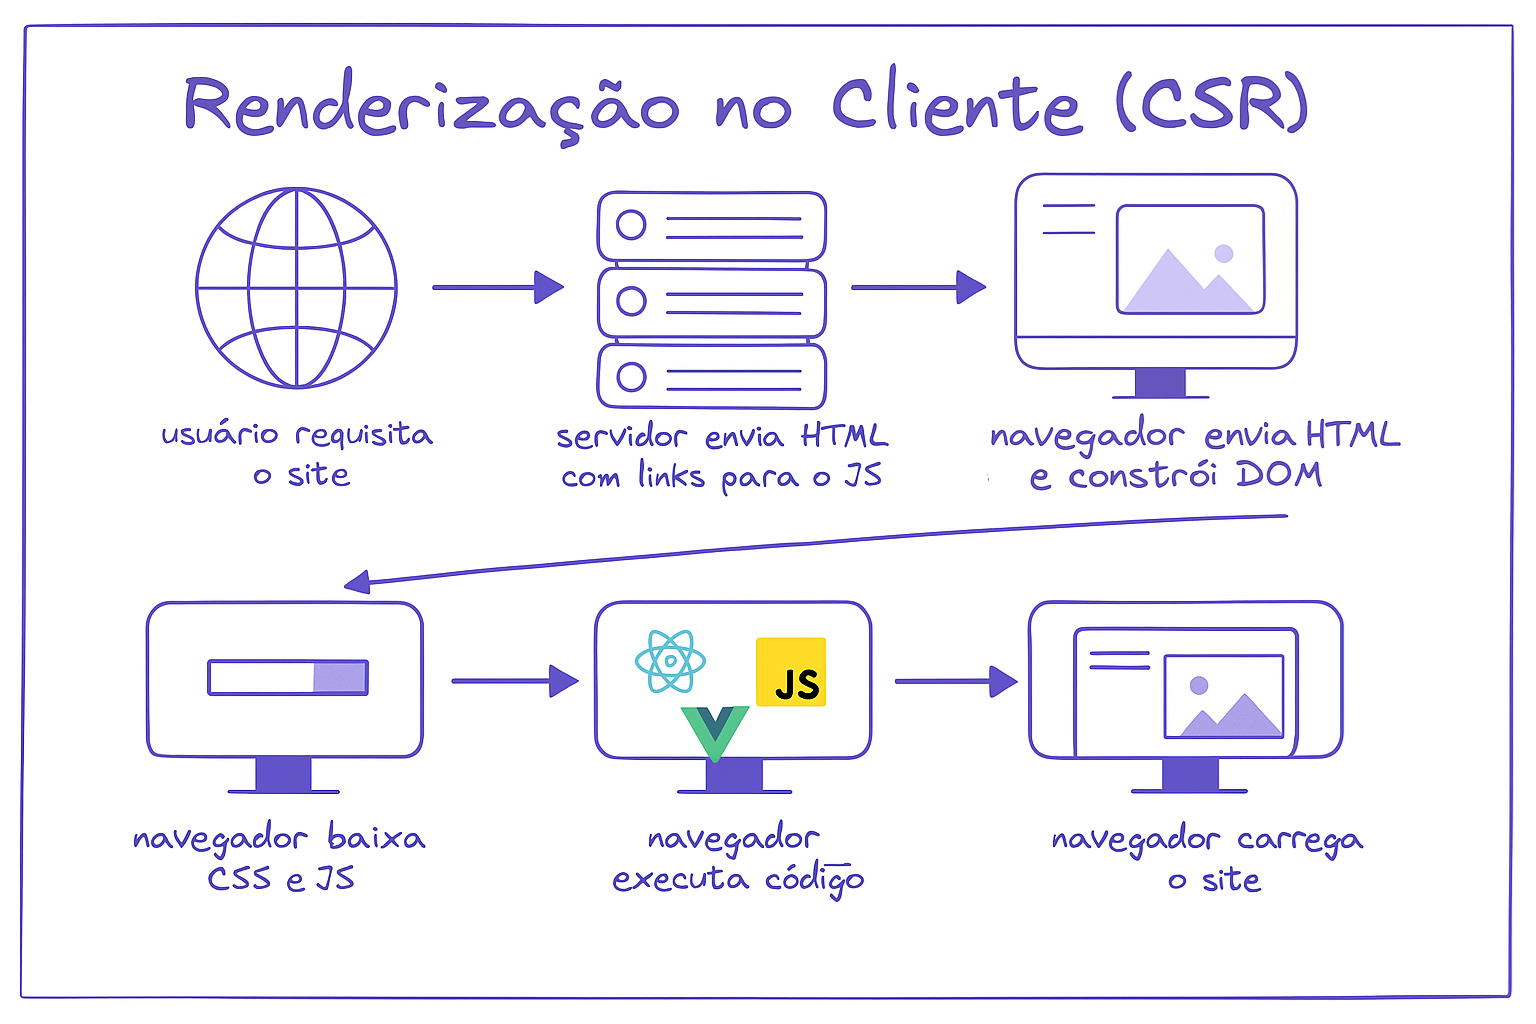
\includegraphics[width=0.9\textwidth]{media/client_side_rendering.png}
    \legend{Fonte: \cite{atori2024} (adaptado)}
    \label{fig:client_side_rendering}
\end{figure}

A \autoref{fig:client_side_rendering} ilustra visualmente o fluxo completo da renderização no lado do cliente (\acrshort{csr}). O processo é iniciado quando o usuário acessa o site em questão. Em resposta, o servidor envia o arquivo \acrshort{html} básico, contendo apenas links para os arquivos de estilo \acrshort{css} e scripts JavaScript responsáveis por carregar e renderizar o conteúdo da aplicação.

Na sequência, o navegador interpreta esse \acrshort{html} e constrói a estrutura da página por meio da árvore \acrshort{dom}. No entanto, o conteúdo principal ainda não está visível. O navegador então precisa baixar os arquivos de estilo (\acrshort{css}) e os scripts JavaScript referenciados no documento inicial.

Com os scripts carregados, o navegador executa o código JavaScript, que normalmente utiliza bibliotecas ou frameworks como React ou Vue para gerar dinamicamente o conteúdo da aplicação. Somente após essa etapa o conteúdo completo do site é finalmente exibido ao usuário, quando o navegador conclui o processo de renderização e o site é carregado completamente.

\begin{lstlisting}[language=html, caption={Exemplo de HTML mínimo em aplicação Angular com CSR}, label={lst:angular_html}]
<!DOCTYPE html>
<html lang="en">
<head>
  <meta charset="utf-8">
  <title>CryptoWebsite</title>
  <base href="/">
  <meta name="viewport" content="width=device-width, initial-scale=1">
  <link rel="icon" type="image/x-icon" href="favicon.ico">
  <style>*,*:before,*:after{margin:0;padding:0;box-sizing:border-box;
    font-family:Inter,sans-serif}html{font-size:62.5%}</style>
  <link rel="stylesheet" href="styles.9d4c7581c7242.css">
</head>
<body>
  <app-root></app-root>
  <script src="runtime.6170988ad52a05db.js" type="module"></script>
  <script src="polyfills.574970d5ec4bdb97.js" type="module"></script>
  <script src="main.202d37bb6740400e.js" type="module"></script>
</body>
</html>
\end{lstlisting}

Esse padrão é típico de aplicações \acrshort{spa}, onde todo o conteúdo é inserido dinamicamente a partir da execução dos arquivos JavaScript. O elemento \texttt{<app-root>} funciona como ponto de entrada da aplicação, sendo substituído no navegador pelos componentes definidos no framework Angular. {\cite{atori2024}}


\section{S2} 
\label{s2}


